\section{Conclusion}
\label{sec:conclusion}

We were successful in implementing an AI agent which was able to score an average reward of more than 200 for 100 consecutive episodes and compared different variants of DQN. DQN was applied effectively on this specific problem, and produced successful results. The success strengthens the use and generality of this algorithm on other problems. We tried it on "CartPole-v1" game defined on openAI gym platform. Our AI agent successfully learnt the game and consecutively won it. This proves the generality of the algorithm.

\begin{figure}[!ht]
%\begin{figure}%
%\vspace*{\fill}
\centering
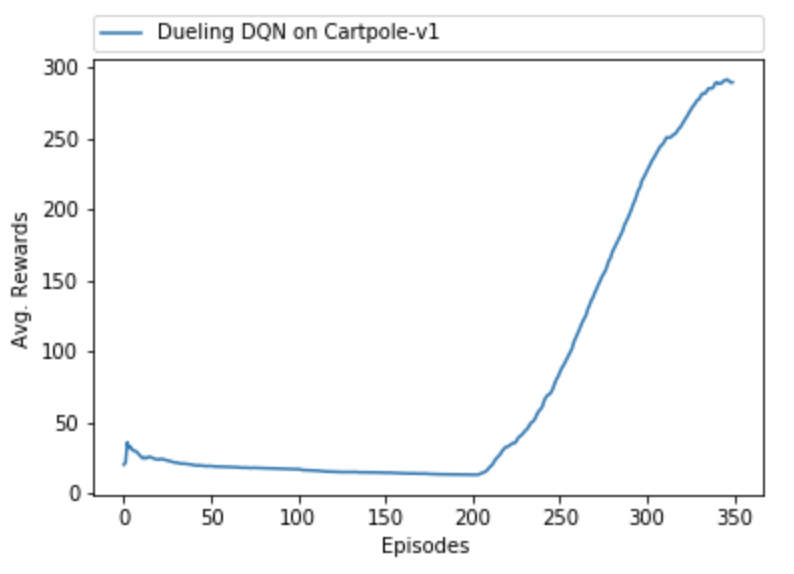
\includegraphics[scale=0.75,width=0.75\columnwidth]{figures/Cartpolev1.png}%
\caption{ Agent learning CartPole Game}%
\label{fig:Visualization}%
\end{figure}
%\vfill}

An agent with too high of a discount was unable to credit actions to success, far enough in the future. Simply put, it was too myopic. As a result, agents learned how to hover, but never learned how to land. We also observed effect of having smaller replay-memory size. Sometimes a drop in the rewards after model learns is because after many consecutive successes, the replay buffer won't have many failure cases to train on. So, it used to 'forget' how to recover from many failure cases.

The DQN variants we tried gave very good results once the hyperparameters were tuned correctly. When implemented the algorithm code in a modularized format, we could easily change the parameters and play with it. Also, minimal tweaks were required for each the DQN variant. Not much of hyperparameter tuning was required across DQN variants. The more advanced Duel Q-learning learner undoubtedly increased the accuracy of the reinforcement learning agent. Given more time and resources, the agent could have been tuned via a more exhaustive grid search. After some literature review, we tried out DQN with Prioritized replay as well. Unfortunately, the results were not promising in comparison to rest of the three approaches. 